% !TEX root = report_kadai3.tex
%% =============================================================
%%  計算機科学実験4 画像認識 レポート（課題3）
%%  ※ 課題2レポート（main.tex）からの差分のみを記載する
%%
%%  【コンパイル方法】LuaLaTeX（report/latexmkrc で指定済み）
%%   ・VS Code：このファイルを保存すると自動でコンパイルされる
%%   ・コマンド：report フォルダで latexmk report_kadai3.tex
%%   ・PDF は report/build/report_kadai3.pdf に出来る
%%   ・表と図の数値は verification/kadai3_compare.py で再現できる
%% =============================================================
\documentclass[a4paper,11pt]{ltjsarticle}

%% ---------- パッケージ ----------
\usepackage[T1]{fontenc}  % コード中の " などを正しく出す（upquote に必要）
\usepackage{lmodern}      % T1 用のきれいな欧文フォント
\usepackage[margin=25mm]{geometry}
\usepackage{amsmath,amssymb,bm}
\usepackage{graphicx}
\usepackage{booktabs}
\usepackage{array}      % 表の列を左寄せにする（>{\raggedright}）ため
\usepackage{xcolor}
\usepackage{listings}   % LuaLaTeX なら日本語と英数字が混ざったコメントも正しく出る
\usepackage{caption}
\usepackage{float}      % [H] で表を書いた位置に固定する
\usepackage[hidelinks]{hyperref}

%% 表の中の文章を左寄せにする列（両端揃えで文字間が空くのを防ぐ）
\newcolumntype{L}[1]{>{\raggedright\arraybackslash}p{#1}}

%% ---------- ソースコードの見た目 ----------
\definecolor{codebg}{HTML}{F7F7F9}
\definecolor{codeframe}{HTML}{D0D0D8}
\definecolor{codekw}{HTML}{0033B3}
\definecolor{codekw2}{HTML}{871094}
\definecolor{codestr}{HTML}{067D17}
\definecolor{codecom}{HTML}{8C8C8C}
\definecolor{codenum}{HTML}{A0A0A0}

\lstdefinestyle{python}{
  language=Python,
  backgroundcolor=\color{codebg},
  frame=single,
  rulecolor=\color{codeframe},
  framesep=4pt,
  xleftmargin=2.2em,
  framexleftmargin=2.2em,
  basicstyle=\ttfamily\small,
  keywordstyle=\color{codekw}\bfseries,
  keywordstyle=[2]\color{codekw2},
  morekeywords=[2]{np,mnist,plt,self,True,False,None},
  stringstyle=\color{codestr},
  commentstyle=\color{codecom},
  numbers=left,
  numberstyle=\scriptsize\color{codenum},
  numbersep=8pt,
  showstringspaces=false,
  tabsize=4,
  breaklines=true,
  breakatwhitespace=false,
  postbreak=\mbox{\textcolor{codenum}{$\hookrightarrow$}\space},
  columns=fullflexible,
  keepspaces=true,
  upquote=true,
  captionpos=t,
}
\lstset{style=python}

%% リファクタリング前後の比較用（前：赤系、後：緑系の背景）
\definecolor{beforebg}{HTML}{FFF5F5}
\definecolor{beforeframe}{HTML}{E8B4B4}
\definecolor{afterbg}{HTML}{F3FBF4}
\definecolor{afterframe}{HTML}{A8D5B0}
\lstdefinestyle{before}{style=python, backgroundcolor=\color{beforebg}, rulecolor=\color{beforeframe}}
\lstdefinestyle{after}{style=python, backgroundcolor=\color{afterbg}, rulecolor=\color{afterframe}}
\renewcommand{\lstlistingname}{ソースコード}
\renewcommand{\lstlistlistingname}{ソースコード一覧}

%% 未記入箇所を目立たせるマクロ（提出前に \todo を全て消すこと）
\newcommand{\todo}[1]{\textcolor{red}{【TODO: #1】}}

%% ソースファイルを読み込む。ファイルが無くてもエラーで止まらず、赤字で知らせる
%%   使い方： \inputcode{style=after, caption={説明}}{src/ファイル名.py}
\newcommand{\inputcode}[2]{%
  \IfFileExists{#2}%
    {\lstinputlisting[#1]{#2}}%
    {\par\todo{\texttt{\detokenize{#2}} が見つかりません。src フォルダに置いてください}\par}}

%% ---------- 表紙情報 ----------
\title{計算機科学実験及演習4 画像認識\\レポート（課題3）}
\author{}
\date{提出期限：\todo{提出期限} \quad 提出日：\today}

\begin{document}
\maketitle
\tableofcontents
\newpage

%% =============================================================
\section{はじめに}
%% =============================================================
本レポートでは、課題2で作成したミニバッチ対応の3層ニューラルネットワークに、誤差逆伝播法による学習の機能を追加したプログラム（課題3）について報告する。
課題1・課題2のレポートと内容が重なる部分（順伝播の計算、ソフトマックス関数、クロスエントロピー誤差など）は省略し、課題2からの差分のみを記載する。

%% =============================================================
\section{課題3：誤差逆伝播法による3層ニューラルネットワークの学習}
%% =============================================================

\subsection{課題内容}
課題2のコードをベースに、3層ニューラルネットワークのパラメータ $W_1, W_2, \bm{b}_1, \bm{b}_2$ を誤差逆伝播法によって学習するプログラムを作成する。
条件は以下の通りである。
\begin{itemize}
  \item ネットワークの構造、バッチサイズは課題2と同じでよい。
  \item 学習には MNIST の学習データ 60000 枚を用いる。
  \item 学習データの枚数を $N$、バッチサイズを $B$ としたとき、$N/B$ 回の繰り返しを1エポックと呼ぶ。1エポック内では学習データ 60000 枚を重複なく利用する。
  \item 学習率 $\eta$ とエポック数は自由に決めてよい。
  \item 各エポックの終了ごとに、1エポック内の平均クロスエントロピー誤差、学習データに対する正答率、テストデータに対する正答率を標準出力に出力する。
\end{itemize}

\subsection{ネットワークの構成}
ネットワークの構造（入力層 784、中間層 $M$、出力層 $C = 10$、活性化関数はシグモイド関数とソフトマックス関数）と順伝播の式は課題2と同じである。
ただし、中間層のノード数は課題2の $M = 500$ から $M = 1000$ に増やした。

\subsubsection{誤差逆伝播法による勾配の計算}
課題2と同様に、$B$ 枚の画像を行方向に並べた行列 $X \in \mathbb{R}^{B \times 784}$ を入力とし、中間層の出力を $Y_1 \in \mathbb{R}^{B \times M}$、出力層の出力を $Y_2 \in \mathbb{R}^{B \times C}$、正解ラベルの one-hot ベクトルを並べた行列を $T \in \{0,1\}^{B \times C}$ とする。
このとき、ミニバッチの平均クロスエントロピー誤差 $E_n$ の各パラメータに対する勾配は、出力層から入力層に向かって順に、次のように計算できる。
\begin{align}
  \Delta_2 &= \frac{\partial E_n}{\partial A_2} = \frac{1}{B}\left(Y_2 - T\right) \in \mathbb{R}^{B \times C}
    && \text{（ソフトマックス関数＋クロスエントロピー誤差）} \label{eq:delta2}\\
  \frac{\partial E_n}{\partial W_2} &= Y_1^{\top} \Delta_2, \qquad
  \frac{\partial E_n}{\partial \bm{b}_2} = \sum_{i=1}^{B} (\Delta_2)_{i,:}
    && \text{（出力層の全結合層）} \label{eq:grad2}\\
  \Delta_1 &= \frac{\partial E_n}{\partial A_1} = \left(\Delta_2 W_2^{\top}\right) \odot Y_1 \odot \left(1 - Y_1\right)
    && \text{（シグモイド関数）} \label{eq:delta1}\\
  \frac{\partial E_n}{\partial W_1} &= X^{\top} \Delta_1, \qquad
  \frac{\partial E_n}{\partial \bm{b}_1} = \sum_{i=1}^{B} (\Delta_1)_{i,:}
    && \text{（中間層の全結合層）} \label{eq:grad1}
\end{align}
ここで $A_1 = X W_1 + \bm{b}_1^{\top}$、$A_2 = Y_1 W_2 + \bm{b}_2^{\top}$ はそれぞれ活性化関数に入る前の値、$\odot$ は要素ごとの積、$(\Delta)_{i,:}$ は $\Delta$ の第 $i$ 行である。
式\eqref{eq:delta1}の $Y_1 \odot (1 - Y_1)$ は、シグモイド関数の微分 $\sigma'(t) = (1 - \sigma(t))\,\sigma(t)$ による。
指導書では各データを列ベクトルとして並べているのに対し、本プログラムでは行方向に並べているため、行列の転置の位置が指導書の式と入れ替わっている。

求めた勾配を用いて、学習率 $\eta$ で各パラメータを次のように更新する。
\begin{equation}
  W_1 \leftarrow W_1 - \eta \frac{\partial E_n}{\partial W_1}, \quad
  \bm{b}_1 \leftarrow \bm{b}_1 - \eta \frac{\partial E_n}{\partial \bm{b}_1}, \quad
  W_2 \leftarrow W_2 - \eta \frac{\partial E_n}{\partial W_2}, \quad
  \bm{b}_2 \leftarrow \bm{b}_2 - \eta \frac{\partial E_n}{\partial \bm{b}_2}
  \label{eq:update}
\end{equation}

\subsubsection{エポックとミニバッチ}
1エポック内で学習データを重複なく使うため、エポックの最初に \texttt{np.random.permutation} で 0～59999 の番号をランダムに並べ替え、その先頭から $B$ 個ずつ取り出してミニバッチとした。
課題2のように毎回 \texttt{np.random.choice} でランダムに選ぶ方法では、1エポック内で同じ画像が何度も選ばれたり、一度も選ばれない画像が出たりするためである。

\subsection{作成したプログラムの説明}
課題2からの変更点を中心に説明する。
プログラムの処理の流れは以下の通りである（リファクタリング後）。
\begin{enumerate}
  \item 重みとバイアスを課題2と同じ方法（平均 0、標準偏差 $1/\sqrt{N}$ の正規乱数）で初期化する。
  \item 学習データ 60000 枚とテストデータ 10000 枚を読み込み、画像を $784$ 次元のベクトルにして画素値を $[0, 1]$ に正規化し、ラベルを one-hot ベクトルに変換する。
  \item 各エポックで以下を行う。
  \begin{enumerate}
    \item 学習データの番号をランダムに並べ替え、先頭から $B = 100$ 枚ずつ取り出す。
    \item 取り出したミニバッチについて、順伝播でクロスエントロピー誤差を計算し、逆伝播で勾配を求め、パラメータを更新する。これを $N/B = 600$ 回繰り返す。
    \item 1エポック内の平均クロスエントロピー誤差と、学習データ・テストデータそれぞれに対する正答率を計算して出力する。
  \end{enumerate}
  \item 全エポックの終了後、誤差と正答率の推移をグラフにして画像として保存する。
\end{enumerate}

課題2から追加・変更した関数を表\ref{tab:func3}に示す。
\begin{table}[H]
  \centering
  \caption{課題3で追加・変更した関数（リファクタリング後）}
  \label{tab:func3}
  \small
  \begin{tabular}{lL{0.62\linewidth}}
    \toprule
    関数名 & 役割 \\
    \midrule
    \texttt{preprocess}      & 【追加】全画像をまとめて $784$ 次元のベクトルにして正規化し、ラベルを one-hot ベクトルに変換する（課題2の \texttt{get\_minibatch} の代わり） \\
    \texttt{init\_params}    & 【追加】重みとバイアスを初期化し、辞書にまとめて返す \\
    \texttt{forward}         & 【変更】順伝播を行い、逆伝播で使う中間層の出力 $Y_1$ も返す \\
    \texttt{backward}        & 【追加】逆伝播を行い、式\eqref{eq:delta2}～\eqref{eq:grad1}により各パラメータの勾配を返す \\
    \texttt{accuracy}        & 【追加】正答率を計算する \\
    \texttt{train\_one\_epoch} & 【追加】ミニバッチを重複なく取り出して1エポック分学習し、平均誤差を返す \\
    \texttt{plot\_history}   & 【追加】誤差と正答率の推移をグラフにして保存する \\
    \texttt{main}            & 【変更】データの読み込みと、エポックの繰り返し、結果の出力を行う \\
    \bottomrule
  \end{tabular}
\end{table}

逆伝播の処理をソースコード\ref{lst:backward}に示す。
式\eqref{eq:delta2}～\eqref{eq:grad1}をそのまま行列演算で書いており、ミニバッチ内の画像を for 文で1枚ずつ処理することはしていない。
\begin{lstlisting}[caption={逆伝播（式\eqref{eq:delta2}～\eqref{eq:grad1}）}, label=lst:backward]
def backward(x, y_true, hidden_layer_activation, y_pred, params):
    #逆伝播を行い、各パラメータの勾配を返す
    output_error = (y_pred - y_true) / y_pred.shape[0] #出力層の誤差 (バッチ内の平均)
    hidden_error = np.dot(output_error, params["W2"].T) * hidden_layer_activation * (1 - hidden_layer_activation) #隠れ層の誤差

    return {
        "W1": np.dot(x.T, hidden_error),
        "b1": np.sum(hidden_error, axis=0),
        "W2": np.dot(hidden_layer_activation.T, output_error),
        "b2": np.sum(output_error, axis=0),
    }
\end{lstlisting}

1エポック分の学習の処理をソースコード\ref{lst:epoch}に示す。
\texttt{perm} から $B$ 個ずつ順に番号を取り出すことで、60000 枚を重複なく使っている。
パラメータの更新（式\eqref{eq:update}）は、パラメータと勾配を同じキーの辞書にしておくことで、1つの for 文で書いた。
\begin{lstlisting}[caption={1エポック分の学習}, label=lst:epoch]
def train_one_epoch(x_train, y_train, params):
    #訓練データを重複なくbatch_size枚ずつ使って1エポック学習し、1エポック内の平均損失を返す
    number_of_sheets = x_train.shape[0] #訓練データの枚数
    iterations_per_epoch = number_of_sheets // batch_size #1エポックあたりのイテレーション数(N/B)

    perm = np.random.permutation(number_of_sheets) #訓練データのインデックスをランダムに並べ替える
    loss_sum = 0.0 #損失の合計値

    for i in range(iterations_per_epoch):
        batch_indices = perm[i * batch_size:(i + 1) * batch_size] #バッチのインデックスを取得
        x_batch = x_train[batch_indices] #バッチの入力データ
        y_batch = y_train[batch_indices] #バッチの正解ラベル

        hidden_layer_activation, y_pred = forward(x_batch, params) #順伝播
        loss_sum += cross_entropy(y_batch, y_pred) #損失の合計値に加算

        grads = backward(x_batch, y_batch, hidden_layer_activation, y_pred, params) #逆伝播
        for key in params: #パラメータの更新
            params[key] -= learning_rate * grads[key]

    return loss_sum / iterations_per_epoch
\end{lstlisting}

\subsection{実行結果}
学習の設定を表\ref{tab:setting}に示す。
\begin{table}[H]
  \centering
  \caption{学習の設定}
  \label{tab:setting}
  \begin{tabular}{ll}
    \toprule
    項目 & 値 \\
    \midrule
    中間層のノード数 $M$ & 1000 \\
    バッチサイズ $B$     & 100 \\
    学習率 $\eta$        & 0.01 \\
    エポック数           & 50 \\
    シード値             & 0 \\
    \bottomrule
  \end{tabular}
\end{table}

リファクタリング後のプログラムの出力（最初と最後の数エポック）をソースコード\ref{lst:run3}に示す。
また、エポックごとの誤差と正答率の推移を図\ref{fig:history}に示す。

\begin{lstlisting}[language={}, numbers=none, caption={課題3の実行結果（一部）}, label=lst:run3]
> python layers.py
epoch   1  loss 1.9103  train_acc 0.7559  test_acc 0.7725
epoch   2  loss 1.2781  train_acc 0.8084  test_acc 0.8173
epoch   3  loss 0.9189  train_acc 0.8381  test_acc 0.8484
...
epoch  48  loss 0.3030  train_acc 0.9135  test_acc 0.9160
epoch  49  loss 0.3019  train_acc 0.9140  test_acc 0.9168
epoch  50  loss 0.3010  train_acc 0.9137  test_acc 0.9164
\end{lstlisting}

\begin{figure}[H]
  \centering
  \IfFileExists{fig/kadai3_after.png}%
    {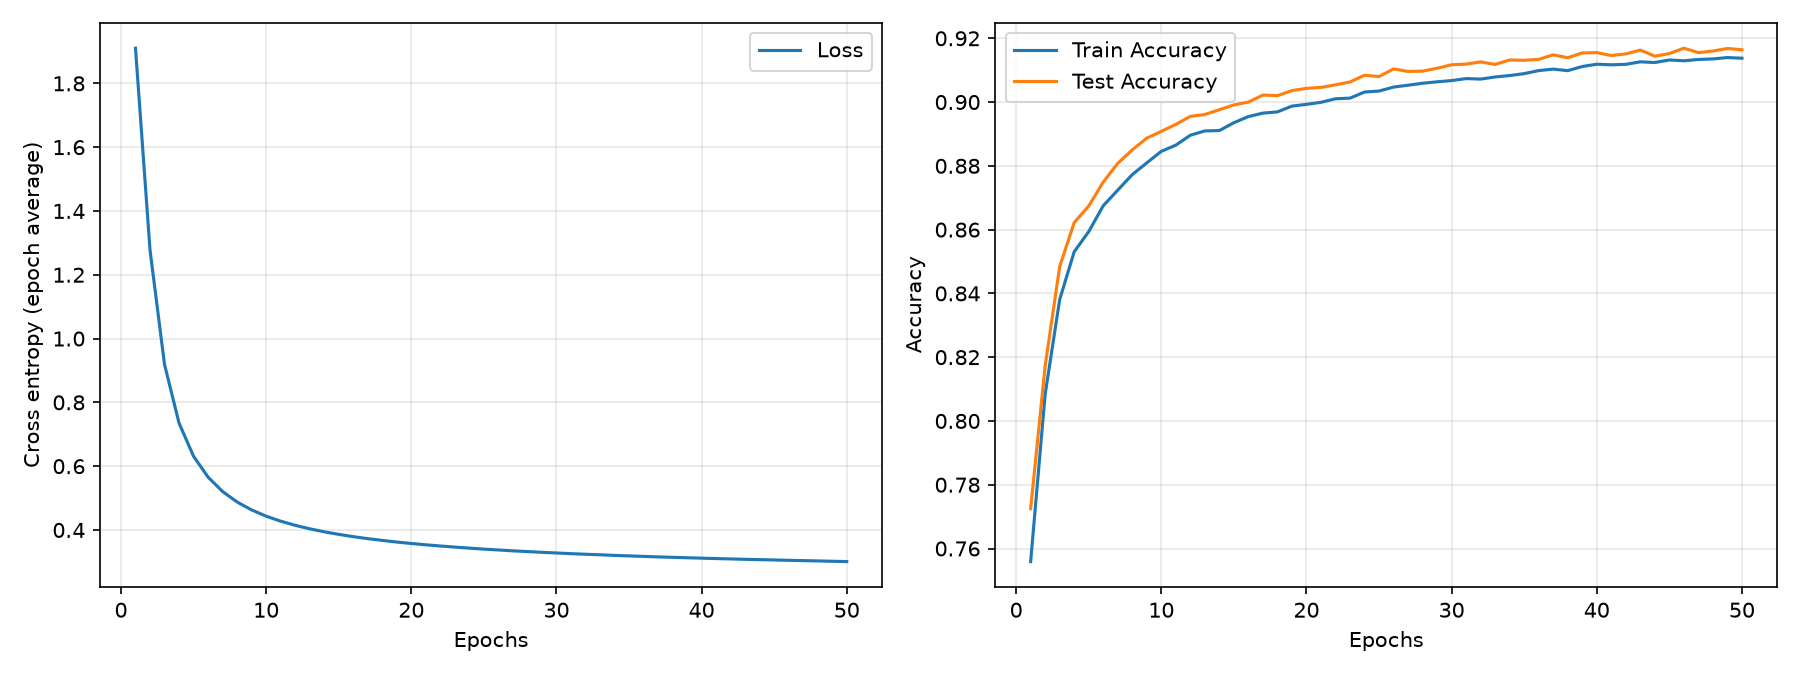
\includegraphics[width=\linewidth]{fig/kadai3_after.png}}%
    {\todo{fig/kadai3\_after.png がありません（verification/kadai3\_compare.py を実行すると作られる）}}
  \caption{リファクタリング後のプログラムの誤差と正答率の推移}
  \label{fig:history}
\end{figure}

学習が進むにつれて誤差は単調に減少し、50エポック後には 0.3010 となった。
正答率は学習データで 91.37\%、テストデータで 91.64\% となり、学習を行っていない課題1・課題2の約 10\% から大きく向上した。
したがって、誤差逆伝播法による勾配の計算とパラメータの更新は正しく動作していると考えられる。

一方で、50エポックの時点でも誤差は減り続けており、正答率もわずかずつ上がり続けている。
また、学習データの正答率がテストデータの正答率よりも低い。
これらのことから、学習がまだ十分に進んでおらず、学習不足の状態であると考えられる。
この原因については、\ref{sec:k3cmp}節で詳しく調べる。

%% -------------------------------------------------------------
\subsection{リファクタリング}
\label{sec:ref3}
%% -------------------------------------------------------------
課題1・課題2と同様に、まず動作するプログラムを作成し（リファクタリング前）、その後コードを見直して改善した（リファクタリング後）。
変更は「構造の改善（振る舞いを変えない）」と「振る舞いを変える改善」に分けて示す。
リファクタリングの方針を決めるにあたっては、課題1・課題2と同様に、生成AIである Claude（Anthropic 社の Opus 5.5 モデル）に改善点を質問し、その提案の意味を理解したうえで適用した。

課題3で行ったリファクタリングを表\ref{tab:ref3}にまとめる。

\begin{table}[H]
  \centering
  \caption{課題3で行ったリファクタリング}
  \label{tab:ref3}
  \small
  \begin{tabular}{L{0.22\linewidth}L{0.36\linewidth}L{0.33\linewidth}}
    \toprule
    手法 & 変更内容 & 目的・効果 \\
    \midrule
    \multicolumn{3}{l}{\textbf{構造の改善（振る舞いを変えない）}} \\
    パラメータの集約 & 4つの変数 \texttt{W1}、\texttt{b1}、\texttt{W2}、\texttt{b2} を、1つの辞書 \texttt{params} にまとめて関数に渡す & 関数の引数を減らして読みやすくする。勾配も同じキーの辞書で返すことで、パラメータの更新を1つの for 文で書ける \\
    関数の抽出 & 重みの初期化を \texttt{init\_params}、1エポック分の学習を \texttt{train\_one\_epoch} に分ける & \texttt{main} を短くし、処理のまとまりごとに名前を付けて流れを分かりやすくする \\
    グローバル変数への依存の除去 & \texttt{backward} の引数 \texttt{batch\_size} をなくし、\texttt{y\_pred.shape[0]} で割る & 課題2の \texttt{cross\_entropy} と同様に、どのバッチサイズでも正しく平均をとれる \\
    変数名の変更 & \texttt{plot\_history} 内のローカル変数 \texttt{epochs} を \texttt{epoch\_axis} に変更 & グローバル変数 \texttt{epochs}（エポック数）と同じ名前で別の意味の変数を作らないようにする \\
    正答率の分割計算 & \texttt{accuracy} で、60000 枚を一度に順伝播せず \texttt{eval\_chunk\_size}（$=10000$）枚ずつ計算する & 中間層の出力（$60000 \times 1000$ 個）を一度に作らず、メモリの使用量を抑える \\
    不要なコードの削除 & コメントアウトして残していた課題2の \texttt{get\_minibatch} を削除 & コードを簡潔にする \\
    \midrule
    \multicolumn{3}{l}{\textbf{振る舞いを変える改善}} \\
    入力の正規化 & \texttt{preprocess} で画素値を \texttt{pixel\_value}（$=255$）で割り、$[0,1]$ にする & リファクタリング前は、コメントには「正規化」と書いていたが、実際には割り算をしていなかった。課題1・課題2と同じ前処理にそろえる \\
    グラフの保存 & \texttt{plot\_history} で、グラフを表示する前に画像ファイルとして保存する & 実行後に結果を見返せるようにする \\
    出力の変更 & 出力するエポック番号を 0～49 から 1～50 に変更 & グラフの横軸（1～50）と番号をそろえる \\
    \bottomrule
  \end{tabular}
\end{table}

主な変更箇所の前後を以下に示す。

\begin{lstlisting}[style=before, caption={【前】パラメータを4つの変数で受け渡す}, label=lst:k3b1]
def backward(x, y_true, hidden_layer_activation, y_pred, W2, batch_size):
    ...
    return dW1, db1, dW2, db2

    #（main 関数内）
    dW1, db1, dW2, db2 = backward(x_batch, y_batch, hidden_layer_activation, y_pred, W2, batch_size) #逆伝播

    #パラメータの更新
    W1 -= learning_rate * dW1
    b1 -= learning_rate * db1
    W2 -= learning_rate * dW2
    b2 -= learning_rate * db2
\end{lstlisting}

\begin{lstlisting}[style=after, caption={【後】パラメータと勾配を辞書で受け渡す}, label=lst:k3a1]
def backward(x, y_true, hidden_layer_activation, y_pred, params):
    ...
    return {"W1": ..., "b1": ..., "W2": ..., "b2": ...}

    #（train_one_epoch 関数内）
    grads = backward(x_batch, y_batch, hidden_layer_activation, y_pred, params) #逆伝播
    for key in params: #パラメータの更新
        params[key] -= learning_rate * grads[key]
\end{lstlisting}

\begin{lstlisting}[style=before, caption={【前】コメントと処理が食い違っている前処理}, label=lst:k3b2]
def preprocess(X, Y):
   #画像を正規化し、ラベルをone-hotベクトルに変換する
   x = X.reshape(X.shape[0], -1).astype(np.float64)
   y = np.eye(class_size)[Y]
   return x, y
\end{lstlisting}

\begin{lstlisting}[style=after, caption={【後】画素値を255で割って正規化する}, label=lst:k3a2]
def preprocess(X, Y):
    #画像を(枚数, 784)にし、ラベルをone-hotベクトルに変換する
    x = X.reshape(X.shape[0], -1).astype(np.float64) / pixel_value #画素値を0〜1に正規化
    y = np.eye(class_size)[Y]
    return x, y
\end{lstlisting}

\subsubsection{変更前後の比較}
\label{sec:k3cmp}
リファクタリングの前後で、学習の結果がどう変わったかを比較した。
比較には、検証用のプログラム \texttt{verification/kadai3\_compare.py} を作成して用いた。
このプログラムは、リファクタリング前後の元のプログラムをそのまま読み込み、エポック数、学習率、正規化の有無だけを差し替えて学習を実行する。
なお、このプログラムは Claude Code を用いて作成した。
実行した学習は次の4通りである（シード値はすべて 0）。
\begin{itemize}
  \item \textbf{A}：リファクタリング前（正規化なし、学習率 0.01）、50エポック
  \item \textbf{B}：リファクタリング後（正規化あり、学習率 0.01）、50エポック
  \item \textbf{C}：リファクタリング後から正規化だけを外した版、3エポック
  \item \textbf{D}：リファクタリング後で学習率を 0.1 にした版（正規化あり）、50エポック
\end{itemize}

\paragraph{構造の改善が振る舞いを変えていないことの確認}
課題2と同様に、乱数を使う順番（$W_1 \to W_2 \to \bm{b}_1 \to \bm{b}_2 \to$ 各エポックの並べ替え）はリファクタリング前と同じにした。
そのため、振る舞いを変える改善である正規化だけを外せば、リファクタリング前と同じ結果になるはずである。
実際に、A と C の最初の3エポックの出力を比較した結果を表\ref{tab:k3same}に示す。

\begin{table}[H]
  \centering
  \caption{リファクタリング前（A）と、後から正規化だけを外した版（C）の比較}
  \label{tab:k3same}
  \small
  \begin{tabular}{clll}
    \toprule
    エポック & 平均誤差 & 学習データの正答率 & テストデータの正答率 \\
    \midrule
    1 & 0.6082010247807045 & 0.9108166666666667 & 0.9124 \\
    2 & 0.3119701394397956 & 0.9297             & 0.9277 \\
    3 & 0.2546080901472541 & 0.94015            & 0.9351 \\
    \bottomrule
  \end{tabular}
\end{table}

3エポックとも、A と C の値は浮動小数点数の全桁まで一致した（表には一致した値を1つだけ示す）。
したがって、パラメータの辞書化や関数の抽出、正答率の分割計算などの構造の改善は、学習の結果を変えていないことが確認できた。

\paragraph{正規化による学習結果の変化}
A、B、D の50エポック後の結果を表\ref{tab:k3cmp}に、エポックごとの推移を図\ref{fig:k3cmp}に示す。

\begin{table}[H]
  \centering
  \caption{リファクタリング前後と学習率による学習結果の比較（50エポック後）}
  \label{tab:k3cmp}
  \small
  \begin{tabular}{llccc}
    \toprule
    & プログラム & 平均誤差 & 学習データの正答率 & テストデータの正答率 \\
    \midrule
    A & 前（正規化なし、$\eta = 0.01$） & 0.0182 & 99.73\% & 96.19\% \\
    B & 後（正規化あり、$\eta = 0.01$） & 0.3010 & 91.37\% & 91.64\% \\
    D & 後（正規化あり、$\eta = 0.1$）  & 0.1108 & 96.99\% & 96.43\% \\
    \bottomrule
  \end{tabular}
\end{table}

\begin{figure}[H]
  \centering
  \IfFileExists{fig/kadai3_learning_rate.png}%
    {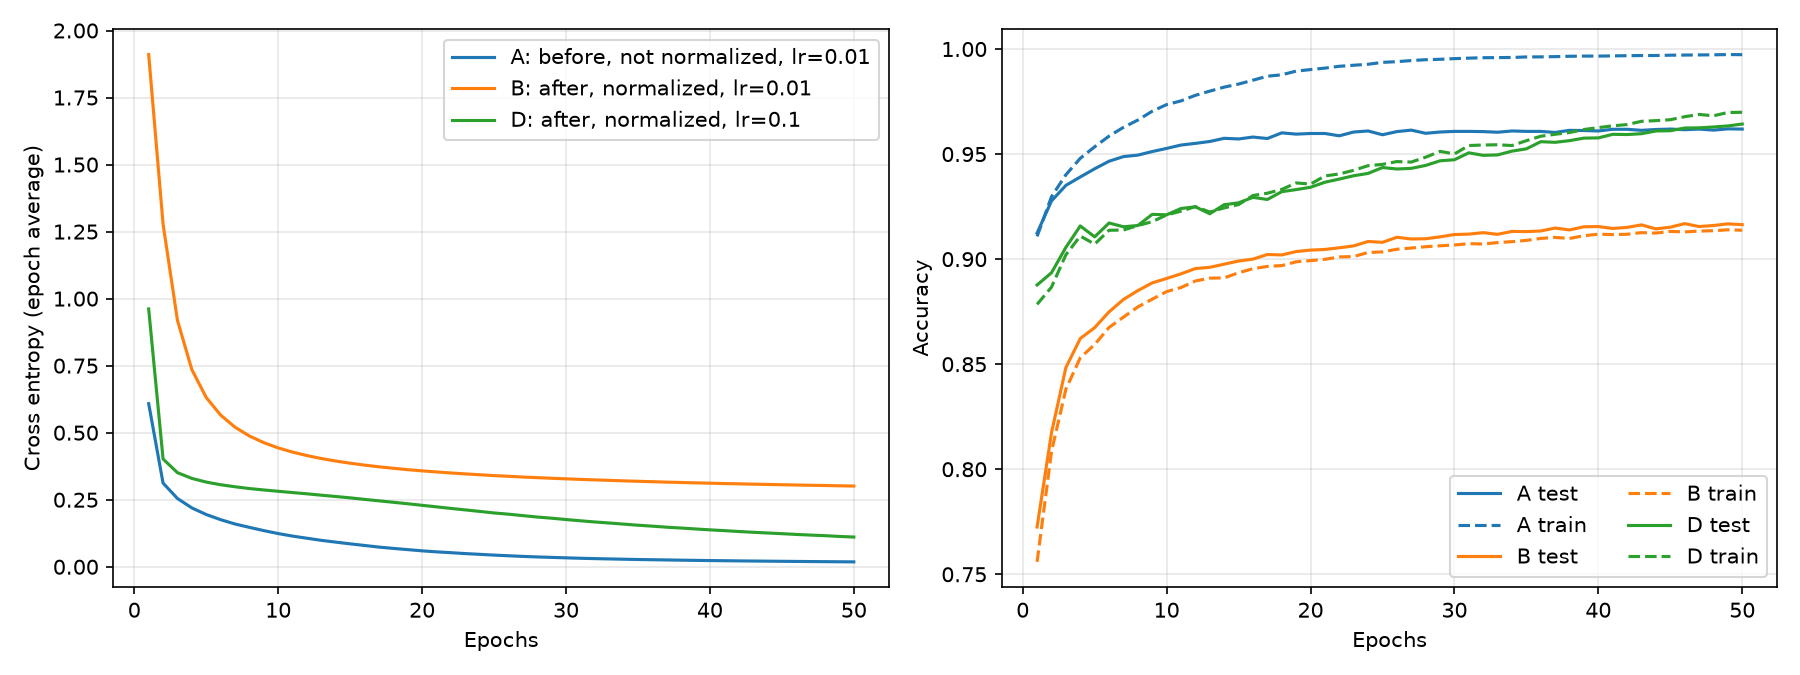
\includegraphics[width=\linewidth]{fig/kadai3_learning_rate.png}}%
    {\todo{fig/kadai3\_learning\_rate.png がありません（verification/kadai3\_compare.py を実行すると作られる）}}
  \caption{A、B、D の誤差（左）と正答率（右）の推移。右図の実線はテストデータ、破線は学習データの正答率}
  \label{fig:k3cmp}
\end{figure}

正規化を加えたリファクタリング後（B）は、リファクタリング前（A）と比べて、テストデータの正答率が 96.19\% から 91.64\% に下がった。
1エポック目の時点でも、A はテストデータの正答率が 91.24\% に達しているのに対し、B は 77.25\% にとどまっており、B は学習の進みが大きく遅い。

この原因は、正規化によって中間層の重み $W_1$ の実質的な学習率が小さくなったためと考えられる。
重み $W_1$ を式\eqref{eq:update}で更新したとき、中間層の入力 $A_1 = X W_1 + \bm{b}_1^{\top}$ が変化する量は、式\eqref{eq:grad1}より
\begin{equation}
  \Delta A_1 = X \cdot \left(-\eta \frac{\partial E_n}{\partial W_1}\right) = -\eta\, X X^{\top} \Delta_1
\end{equation}
となり、入力 $X$ の大きさの2乗に比例する。
画素値を 255 で割らない場合、$X$ は 255 倍大きくなるため、同じ学習率 $\eta = 0.01$ でも $A_1$ の変化量は $255^2 \approx 65000$ 倍になる。
つまり、正規化しない A は、$W_1$ について非常に大きな学習率で学習していたことになり、そのために少ないエポック数で学習が進んだと考えられる。
逆に、正規化した B では、$\eta = 0.01$ が小さすぎて、50エポックでは学習が終わらなかった。

この考えを確かめるため、正規化したまま学習率を10倍の $\eta = 0.1$ にした D を実行した。
D は1エポック目のテストデータの正答率が 88.77\% となり、B（77.25\%）よりも速く学習が進んだ。
50エポック後のテストデータの正答率は 96.43\% となり、A（96.19\%）と同程度まで向上した。

また、A は学習データの正答率が 99.73\% であるのに対し、テストデータの正答率は 96.19\% であり、3.5 ポイントの差がある。
これは、学習データに過剰に適合した過学習の状態であると考えられる。
一方、D の差は 0.56 ポイントと小さく、テストデータの正答率も A よりわずかに高い。
したがって、「正規化しないほうがうまくいく」ように見えたのは、正規化そのものが悪いのではなく、正規化したときに学習率を調整していなかったためであり、正規化したうえで学習率を適切に選ぶのがよいと考える。

%% -------------------------------------------------------------
\subsection{工夫点}
%% -------------------------------------------------------------
\begin{itemize}
  \item \textbf{逆伝播の行列演算による一括計算}：式\eqref{eq:delta2}～\eqref{eq:grad1}を行列演算でそのまま実装し、ミニバッチ内の画像を for 文で1枚ずつ処理しないようにした。
  \item \textbf{重複のないミニバッチの取り出し}：エポックごとに \texttt{np.random.permutation} で番号を並べ替え、先頭から順に $B$ 個ずつ取り出すことで、1エポック内で 60000 枚を重複なく使うようにした。
  \item \textbf{前処理をまとめて1回だけ行う}：正規化と one-hot ベクトルへの変換を、ミニバッチを取り出すたびではなく、学習の前に全データに対して1回だけ行うようにした。
  \item \textbf{パラメータと勾配を辞書で管理}：パラメータと勾配を同じキーの辞書にすることで、関数の引数を減らし、パラメータの更新も1つの for 文で書けるようにした。
  \item \textbf{学習の推移の記録と保存}：エポックごとの誤差と正答率を記録してグラフにし、画像として保存するようにした。これにより、学習がうまく進んでいるか、どの程度で打ち切ってよいかを確認できる。
  \item \textbf{リファクタリング前後の検証}：振る舞いを変える改善（正規化）だけを外した版と比較することで、それ以外の変更が学習の結果を変えていないことを確かめた（\ref{sec:k3cmp}節）。
\end{itemize}

%% -------------------------------------------------------------
\subsection{問題点}
%% -------------------------------------------------------------
\begin{itemize}
  \item \textbf{学習率が正規化した入力に合っていない}：リファクタリング後のプログラムは学習率を $\eta = 0.01$ のままにしているため、50エポックでは学習が終わらず、テストデータの正答率は 91.64\% にとどまる（表\ref{tab:k3cmp}）。学習率を 0.1 にすると 96.43\% まで向上することを確認した。\todo{プログラムの学習率を 0.1 に変更するか決める（kadai3\_after.py に正規化の TODO コメントも残っている）}
  \item \textbf{学習に時間がかかる}：中間層のノード数が 1000 であるため、50エポックの学習に約9分かかる。学習率などの設定を変えて試すたびに長い時間がかかる。
  \item \textbf{エポック数を決める基準がない}：エポック数は 50 に固定しており、学習が十分に進んだかどうかに関係なく終了する。正規化しない場合（A）は、20エポック以降はテストデータの正答率がほとんど上がらない（20エポックで 95.98\%、50エポックで 96.19\%）一方、学習データの正答率は 99.02\% から 99.73\% に上がっており、学習データへの過剰な適合が進んでいた（図\ref{fig:k3cmp}）。テストデータとは別に検証用のデータを分けておき、その正答率が上がらなくなった時点で学習を打ち切るなどの工夫が考えられる。
  \item \textbf{学習したパラメータを保存していない}：学習した重みとバイアスはプログラムの終了とともに失われるため、学習済みのネットワークで認識を行うたびに学習し直す必要がある。
\end{itemize}

%% =============================================================
\section{おわりに}
%% =============================================================
本レポートでは、課題2のプログラムに誤差逆伝播法による学習の機能を追加し、MNIST の学習データ 60000 枚を用いて3層ニューラルネットワークを学習させた。
課題1・課題2では約 10\% だった正答率が、学習によってテストデータで 91.64\%（学習率を 0.1 にした場合は 96.43\%）まで向上した。
また、リファクタリングの前後で学習の結果を比較する中で、入力の正規化と学習率の関係によって学習の進み方が大きく変わることが分かった。

\todo{感想}

%% =============================================================
\appendix
\section{ソースコード}
%% =============================================================
提出したソースファイルの一覧を表\ref{tab:files}に示す。
\begin{table}[H]
  \centering
  \caption{提出ファイル}
  \label{tab:files}
  \begin{tabular}{ll}
    \toprule
    ファイル名 & 内容 \\
    \midrule
    \texttt{kadai3\_before.py} & 課題3（リファクタリング前） \\
    \texttt{kadai3\_after.py}  & 課題3（リファクタリング後） \\
    \bottomrule
  \end{tabular}
\end{table}

\inputcode{style=before, caption={課題3のプログラム（リファクタリング前）}, label=lst:k3before}{src/kadai3_before.py}
\inputcode{style=after,  caption={課題3のプログラム（リファクタリング後）}, label=lst:k3after}{src/kadai3_after.py}

\end{document}
